\newpage\setcounter{dang}{0}
\section{TÍCH VÔ HƯỚNG CỦA HAI VECTƠ}
\subsection{Tóm tắt lí thuyết}
\subsubsection{Góc giữa hai vectơ }
\immini
{
		Cho hai vectơ $\vec{u}$ và $\vec{v}$ khác $\vec{0}$. Từ một điểm $A$ tùy ý, vẽ các vectơ $\vec{AB}=\vec{u}$. Khi đó, số đo của góc $BAC$ được gọi là số đo góc giữa hai vectơ  $\vec{u}$ và $\vec{v}$ hay đơn giản là góc giữa hai vectơ $\vec{u}$, $\vec{v}$.\\ Kí hiệu là $\left(\vec{u},\vec{v}\right)$.
}
{
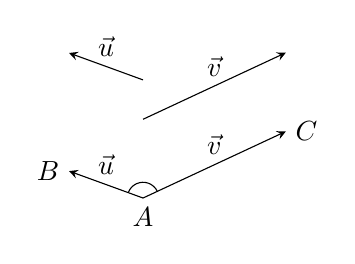
\begin{tikzpicture}[>=stealth]
	\path (160:1cm) coordinate (B);
	\path (B)++(0,1.5) coordinate (B');
	\path (25:2cm) coordinate (C);
	\path (C)++(0,1) coordinate (A');
	\draw[->] (0,1.5) -- (B') node[above,midway]{$\vec{u}$};
	\draw[->] (0,1) -- (A') node[above,midway]{$\vec{v}$};
	\draw[->] (0,0) node[below]{$A$} -- (B) node[left]{$B$} node[above,midway]{$\vec{u}$};
	\draw[->] (0,0) -- (C) node[right]{$C$} node[above,midway]{$\vec{v}$};
	\draw (25:0.2cm) arc (25:160:0.2);
\end{tikzpicture}
}
\begin{note}
	\begin{itemize}
		\item Quy ước rằng góc giữa hai vectơ $\vec{u}$ và $\vec{0}$ có thể nhận một giá trị tùy ý từ $0^\circ$ đến $180^\circ$.
		\item Nếu $\left(\vec{u},\vec{v}\right)=90^\circ$ thì ta nói rằng  $\vec{u}$ và $\vec{v}$ vuông góc với nhau, kí hiệu là $\vec{u} \perp \vec{v}$ hoặc $\vec{v} \perp \vec{u}$. \\
		Đặc biệt $\vec{0}$ được coi là vuông góc với mọi vectơ.
	\end{itemize}
\end{note}

\begin{vd}%[0H2B2]
	Cho tam giác $ABC$ vuông tại $A$ có $\widehat{B}=60^\circ$. Tính $\left(\vec{AB},\vec{AC}\right)$,$\left(\vec{CA},\vec{CB}\right)$, $\left(\vec{AB},\vec{BC}\right)$.
	\loigiai{
		\immini{Ta có \\
$\left(\vec{AB},\vec{AC}\right)=\widehat{BAC}=90^\circ$\\ $\left(\vec{CA},\vec{CB}\right)=\widehat{ACB}=30^\circ$ \\
$\left(\vec{AB},\vec{BC}\right)=\left(\vec{BD},\vec{BC}\right)=\widehat{DBC}=120^\circ$
}{
			\begin{tikzpicture}[>=stealth, line join=round, line cap=round, font=\footnotesize, scale=0.7]
			\coordinate[label=below left:$A$](A) at (0,0);
			\coordinate[label=below right:$B$](B) at (2,0);
			\coordinate[label=above right:$C$](C) at (0,4);
			\coordinate[label=below :$D$](D) at (4,0);
			\draw[dashed] (B)--(D);
			\draw (A)--(B)--(C)--cycle ;
			\path pic[draw,blue,angle radius=4mm] {angle = C--B--A} (B)--($(B)!8mm!($($(B)!8mm!(C)$)!.5!($(B)!8mm!(A)$)$)$)node[scale=1,pos=1]{$60^\circ$};
			\foreach \x/\y/\z in {C/A/B} {
				\path
				($(\y)!5pt!(\z)$) coordinate (1)
				($(\y)!5pt!(\x)$) coordinate (2)
				($(1)+(2)-(\y)$) coordinate (3)

				;
				\draw (1)--(3)--(2); }
			\foreach \x in {A,B,C,D}
			\draw[fill=black] (\x) circle (1pt);
			\end{tikzpicture}
		}
	}
\end{vd}
\subsubsection{Tích vô hướng của hai vectơ}
	Tích vô hướng của hai vectơ $\vec{u}$ và $ \vec{v}$ là một số, kí hiệu là $\vec{u}\cdot \vec{v}$, được xác định bởi công thức sau:
	$$\vec{u}\cdot \vec{v} = \left|\vec{u}\right|\left|\vec{v}\right| \cos\left(\vec{u},\vec{v}\right).$$
\begin{note}
	\begin{itemize}
		\item $\vec{u}\perp \vec{v} \Leftrightarrow \vec{u}\cdot \vec{v}=0$.
		\item $\vec{u} \cdot \vec{u}$ còn được viết là $\vec{u}^2$ và được coi là bình phương vô hướng của vectơ $\vec{u}$. Ta có $\vec{u}^2=\left|\vec{u}\right|\left|\vec{u}\right| \cos 0^\circ = \left|\vec{u}\right|^2$.
	\end{itemize}
\end{note}
\begin{vd}%[0H2B2]
	Cho hình vuông $ABCD$ cạnh bằng $2a\sqrt{2}$. Tính tích vô hướng $\vec{AB}\cdot \vec{AC}.$
	\loigiai{
		\immini{
			Ta có $\vec{AB}\cdot\vec{AC}=\left|\vec{AB}\right|\cdot\left|\vec{AC}\right|\cdot\cos\left(\vec{AB},\vec{AC}\right).$\\
			Vì tam giác $ABC$ vuông tại $A$ nên
			\\ $AC^2=AB^2+BC^2=\left(2a\sqrt{2}\right)^2+\left(2a\sqrt{2}\right)^2=16a^2$
			$\Rightarrow AC=4a.$\\
			 Suy ra $\vec{AB}\cdot\vec{AC}=2a\sqrt{2}\cdot4a\cdot\cos 45^\circ=8a^2.$
		}
		{

	\begin{tikzpicture}[>=stealth, line join=round, line cap=round, font=\footnotesize, scale=0.7]
	%
	\coordinate[label=below left:$A$](A) at (0,0);
	\coordinate[label=below right:$B$](B) at (3,0);
	\coordinate[label=above right:$C$](C) at (3,3);
	\coordinate[label=above left:$D$](D) at (0,3);
	\draw (A)--(B)--(C)--(D)--cycle (A)--(C) ;
	\draw[line width=0.4pt,black] (A)--(D)node[left,pos=0.5]{$2a\sqrt{2}$};
	\draw pic[angle radius=5mm,draw=black,"$45^\circ$",angle eccentricity=2] {angle = B--A--C};

	\foreach \x in {A,B,C,D}
	\draw[fill=black] (\x) circle (1pt);

\end{tikzpicture}		}
	}
\end{vd}
\subsubsection{Biểu thức tọa độ và tích chất của tích vô hướng}
	Tích vô hướng của hai vectơ $\vec{u}=\left(x;y\right)$ và $\vec{v}=\left(x';y'\right)$ được tính theo công thức
	$$\vec{u} \cdot \vec{v} = xx'+yy'.$$
\begin{nx}
	\textbf{}
\begin{itemize}
	\item Hai vectơ $\vec{u}$ và $\vec{v}$ vuông góc với nhau khi và chỉ khi $xx' + yy'=0$.
	\item Bình phương vô hướng của $\vec{u}(x;y)$ là $\vec{u}^2=x^2+y^2$.
	\item Nếu $\vec{u} \ne \vec{0}$ và $\vec{v}\ne \vec{0}$ thì $$\cos \left(\vec{u},\vec{v}\right)=\dfrac{\vec{u}\cdot \vec{v}}{\left| \vec{u}\right|\cdot \left| \vec{v}\right|}=\dfrac{xx'+yy'}{\sqrt{x^2+y^2}\cdot \sqrt{x'^2+y'^2}}.$$
\end{itemize}
\end{nx}

\begin{vd}%[0H2B2]
	Cho các vectơ $\overrightarrow{a}=-\overrightarrow{i}+\overrightarrow{j}, \overrightarrow{b}=\overrightarrow{i}+3\overrightarrow{j}$. Tính tích vô hướng và tìm góc giữa hai vectơ $\overrightarrow{a}$ và $\overrightarrow{b}$.
	\loigiai{
		Ta có $\vec{a}=(-1;1), \vec{b}=(1;3)$.
\begin{itemize}
\item $\vec{a}\cdot \vec{b}=-1\cdot 1 + 1\cdot 3= 2.$
	\item 	$\cos (\overrightarrow{a},\overrightarrow{b})=\dfrac{\overrightarrow{a}\cdot\overrightarrow{b}}{|\overrightarrow{a}|\cdot|\overrightarrow{b}|}=\dfrac{2}{\sqrt{(-1)^2+1^2}\cdot\sqrt{1^2+3^2}}=\dfrac{2}{2\sqrt{5}}=\dfrac{1}{\sqrt{5}}$.\\
	Do đó góc giữa hai vectơ $\overrightarrow{a}$ và $\overrightarrow{b}$ bằng $\alpha \in [0^\circ;180^\circ]$ mà $\cos \alpha =\dfrac{1}{\sqrt{5}}$.
\end{itemize}

	}
\end{vd}


\begin{tc}
	Với ba vectơ $\vec{u},\vec{v},\vec{w}$ bất kì và mọi số thực $k$ ta có
	\begin{itemize}
		\item $\vec{u}\cdot \vec{v}=\vec{v}\cdot \vec{u}$ (tính chất giao hoán)
		\item $\vec{u} \cdot \left(\vec{v}+\vec{w}\right)=\vec{u}\cdot \vec{v}+\vec{u}\cdot \vec{w}$ (tính chất phân phối với phép cộng)
		\item $\left(k\vec{u}\right)\vec{v}=k\left(\vec{u}\cdot \vec{v}\right)=\vec{u}\cdot \left(k\vec{v}\right)$.
	\end{itemize}
\end{tc}
\begin{note}
	Từ các tính chất trên ta có thể chứng minh được
	\begin{itemize}
		\item $\vec{u} \cdot \left(\vec{v}-\vec{w}\right)=\vec{u}\cdot \vec{v}-\vec{u}\cdot \vec{w}$ (tính chất phân phối với phép trừ)
		\item $\left(\vec{u}+\vec{v}\right)^2=\vec{u}^2+2\vec{u}\cdot\vec{v} +\vec{v}^2; \left(\vec{u}-\vec{v}\right)^2=\vec{u}^2-2\vec{u}\cdot\vec{v} +\vec{v}^2 $
		\item $\left(\vec{u}+\vec{v}\right)\left(\vec{u}-\vec{v}\right)=\vec{u}^2-\vec{v}^2$
	\end{itemize}
\end{note}

\begin{vd}%[0H2G2]
	Cho hình vuông $ABCD$ tâm $O$. Tìm tập hợp các điểm $M$ thỏa mãn $$ MA^2+MB^2+MC^2=3MD^2.$$
	\loigiai{
		\immini{Ta có\\
			$MA^2 + MB^2 + MC^2 = 3MD^2 $\\
			$\Leftrightarrow \vec{MA}^2+\vec{MB}^2+\vec{MC}^2=3\vec{MD}^2$\\
			$\Leftrightarrow \left(\vec{MO}+\vec{OA}\right)^2~+~\left(\vec{MO}+\vec{OB}\right)^2~+~\left({\vec{MO}+\vec{OC}}\right)^2~=~3~{\left(\vec{MO}+\vec{OD}\right)^2}$\\
			$ \Leftrightarrow \vec{MO}\cdot \left(\vec{OA}+\vec{OB}+\vec{OC}-3\vec{OD}\right)=0 $\\
			$\Leftrightarrow \vec{MO}\cdot\left(\vec{DA}+\vec{DB}+\vec{DC}\right) = 0$\\
			$ \Leftrightarrow \vec{MO} \cdot\vec{DB}  = 0$ (vì $\vec{DA}+\vec{DC}=\vec{DB}$).\\
			$ \Leftrightarrow \hoac{&\vec{MO}= \vec{0}
				\\&MO \perp DB.}$
			\\ Vậy tập hợp các điểm $M$ là đường thẳng $AC.$
		}
		{

	\begin{tikzpicture}[>=stealth, line join=round, line cap=round, font=\footnotesize, scale=0.7]
%
		\coordinate[label=below left:$A$](A) at (0,0);
		\coordinate[label=below right:$B$](B) at (3,0);
		\coordinate[label=above right:$C$](C) at (3,3);
		\coordinate[label=above left:$D$](D) at (0,3);
		\coordinate[label=left:$O$] (O) at ($(A)!0.5!(C)$);
		\draw (A)--(B)--(C)--(D)--cycle (A)--(C) (B)--(D);
 \foreach \x/\y/\z in {A/O/B} {
 	\path
 	($(\y)!5pt!(\z)$) coordinate (1)
 	($(\y)!5pt!(\x)$) coordinate (2)
 	($(1)+(2)-(\y)$) coordinate (3)

 	;
 	\draw (1)--(3)--(2); }


		 \foreach \x in {A,B,C,D,O}
		\draw[fill=black] (\x) circle (1pt);

			\end{tikzpicture}
		}


	}
\end{vd}



\subsection{Các dạng toán thường gặp}

\begin{dang}{Xác định góc giữa hai vectơ}
	\immini
	{
		Cho hai vectơ $\overrightarrow{a}$ và $\overrightarrow{b}$ khác $\overrightarrow{0}$. Khi đó để xác định góc giữa hai vectơ ta thực hiện như sau:
		\begin{itemize}
			\item Vẽ vectơ $\overrightarrow{OA} = \overrightarrow{a}$; $\overrightarrow{OB} = \overrightarrow{b}$.
			\item Khi đó góc giữa $\overrightarrow{a}$ và $\overrightarrow{b}$ là $\left(\overrightarrow{a}, \overrightarrow{b}\right) = \widehat{AOB}$.
		\end{itemize}
	 \textbf{\textit{$\ast$ Chú ý}}
		\begin{itemize}
			\item $0\leq \left(\overrightarrow{a}, \overrightarrow{b}\right)\leq 180^\circ$.
			\item $\left(\overrightarrow{a}, \overrightarrow{b}\right) = 0^\circ \Leftrightarrow \overrightarrow{a} \text{ và } \overrightarrow{b}$ cùng hướng.
			\item $\left(\overrightarrow{a}, \overrightarrow{b}\right) = 180^\circ \Leftrightarrow \overrightarrow{a} \text{ và } \overrightarrow{b}$ ngược hướng.
		\end{itemize}
	}
	{
		\begin{tikzpicture}[line cap=round, line join= round, scale=1, font=\footnotesize, >=stealth]
			\draw[->] (0,0)node[left]{$O$} coordinate (O)--(2,1)node[right]{$A$} coordinate (A);
			\draw[->] (O) --(2,-2)node[right]{$B$} coordinate (B);
			\draw[->] (0,1) --node[pos=.5, above]{$\overrightarrow{a}$}(2,2);
			\draw[->] (-.5,-1) --node[rotate=-30,pos=.5, above]{$\overrightarrow{b}$}(1.5,-3);
			\draw[dashed] (-.5,-1)--(O)--(0,1) (2,2)--(A) (1.5,-3)--(B);
			\draw pic[draw, angle radius=2mm, angle eccentricity=2,"$\alpha$"]{angle=B--O--A};
		\end{tikzpicture}
	}
\end{dang}
\begin{vd}%[0H2Y2-1]
	Góc $\widehat{N}$ trong $\triangle MNP$ được biểu diễn theo hai vectơ nào? Viết kí hiệu.
\loigiai{
	\immini
	{
		Góc $\widehat{N}$ trong $\triangle MNP$ được biểu diễn theo hai vectơ $\overrightarrow{NM}$ và $\overrightarrow{NP}$.
		\\
		Ta có $\widehat{MNP} = \left(\overrightarrow{NM}, \overrightarrow{NP}\right)$.
	}
	{
		\begin{tikzpicture}[scale=1, line cap=round, line join=round, font=\footnotesize, >=stealth]
			\draw[->] (0,0)node[left]{$N$} coordinate (N)--(2,1)node[above right]{$M$}coordinate (M);
			\draw[->] (0,0)--(3,-1)node[right]{$P$}coordinate (P);
			\draw (2,1)--(3,-1)
			pic[draw, angle radius=2mm, angle eccentricity=2,"$\alpha$"]{angle=P--N--M};
		\end{tikzpicture}
	}
}
\end{vd}

\begin{vd}%[0H2Y2-1]
	Góc tạo bởi hai vectơ $\overrightarrow{OX}$ và $\overrightarrow{XY}$ là góc nào trong hình bình hành $OXYZ$?
\loigiai{
	\immini
	{
		Do $OXYZ$ là hình bình hành nên ta có $\overrightarrow{XY}=\overrightarrow{OZ}$.
		\\
		Suy ra $\left(\overrightarrow{OX}, \overrightarrow{XY}\right)=\left(\overrightarrow{OX}, \overrightarrow{OZ}\right) = \widehat{XOZ}$.
	}
	{
		\begin{tikzpicture}[line cap=round, line join=round, scale=1, font=\footnotesize, >=stealth]
			\draw[->] (0,0) coordinate (O)--(3,0) coordinate (X);
			\draw[->] (O)--(1,2) coordinate (Z);
			\draw[->] (O)--($(X)-(O)+(Z)$) coordinate (Y);
			\draw (Z)--(Y)--(X);
			\foreach \a/\b in {O/200,X/0,Y/30,Z/110} \fill[black] (\a)circle(.7pt) ($(\a)+(\b:3mm)$)node[scale=.8]{$\a$};
		\end{tikzpicture}
	}
}
\end{vd}

\begin{vd}%[0H2B2-1]
	Cho tam giác đều $ABC$. Tính $P=\cos\left(\vec{AB},\vec{BC}\right)$.
	\loigiai{
		\immini
		{
			Vẽ $\vec{BE}=\vec{AB}$. Khi đó, ta có
			\begin{eqnarray*}
				\left(\vec{AB},\vec{BC}\right)&=&\left(\vec{BE},\vec{BC}\right) \\
				&=&\widehat{CBE} \\
				&=&180^\circ-\widehat{CBA}=120^\circ.
			\end{eqnarray*}
			Suy ra $\cos\left(\vec{AB},\vec{BC}\right)=\cos 120^\circ=-\dfrac{1}{2}$.
		}
		{
			\begin{tikzpicture}[>=stealth,line join=round,line cap=round,font=\footnotesize,scale=1]
				\def\a{3}
				\path
				(0,0) coordinate (A)
				(0:\a) coordinate (B)
				(60:\a) coordinate (C)
				($ (B)+(0:\a) $) coordinate (E);
				\foreach \x/\y in {A/B,B/C,B/E}\draw[->] (\x)--(\y);
				\draw (A)--(C);
				\foreach \x/\g in {A/-90,B/-90,C/90,E/-90}\fill[black] (\x) circle (1pt)+(\g:3mm) node{$ \x $};
			\end{tikzpicture}
		}
	}
\end{vd}

\begin{dang}{Tính tích vô hướng}
	Cho $\overrightarrow{a} = (a_1; a_2)$ và $\overrightarrow{b} = (b_1; b_2)$. Khi đó, ta có công thức
	\fbox{$\overrightarrow{a}.\overrightarrow{b} = a_1\cdot b_1 + a_2\cdot b_2$.}
	\\
	Tích vô hướng còn được tính theo công thức \fbox{$\overrightarrow{a}.\overrightarrow{b}=\left|\overrightarrow{a}\right|\cdot \left|\overrightarrow{b}\right|\cdot \cos \left(\overrightarrow{a}, \overrightarrow{b}\right)$.}
	\\
	$\ast$ \textbf{\textit{Chú ý}} $\overrightarrow{a}\perp \overrightarrow{b} \Leftrightarrow \overrightarrow{a}\cdot \overrightarrow{b} =0$.
\end{dang}

\begin{vd}%[0H2K2-3]
	Cho tam giác $ABC$ có $A(1;2), B(-2;6), C(9;8)$. Tính $\overrightarrow{AB}\cdot \overrightarrow{AC}$. Tam giác $\triangle ABC$ là tam giác gì?
\loigiai{
	Ta có $\overrightarrow{AB} = (-3;4)$, $\overrightarrow{AC}=(8;6) \Rightarrow\overrightarrow{AB}\cdot \overrightarrow{AC} =-3\cdot 8+4\cdot 6=0$.\\
	Do đó $\overrightarrow{AB}\perp \overrightarrow{AC}$ hay tam giác $ABC$ vuông tại $A$.
}
\end{vd}

\begin{vd}%[0H2Y2-2]
	Cho tam giác $ABC$ vuông tại $A$ có $AB=a, BC=2a$ và $G$ là trọng tâm.
	\begin{enumerate}
		\item Tính các tích vô hướng: $\overrightarrow{BA}\cdot\overrightarrow{BC}$; $\overrightarrow{BC}\cdot\overrightarrow{CA}$.
		\item Tính giá trị của biểu thức $\overrightarrow{AB}\cdot\overrightarrow{BC}+\overrightarrow{BC}\cdot\overrightarrow{CA}+\overrightarrow{CA}\cdot\overrightarrow{AB}$.
		\item Tính giá trị của biểu thức $\overrightarrow{GA}\cdot\overrightarrow{GB}+\overrightarrow{GB}\cdot\overrightarrow{GC}+\overrightarrow{GC}\cdot\overrightarrow{GA}$.
	\end{enumerate}
\loigiai{
	\begin{enumerate}
		\item Công thức tích vô hướng $\overrightarrow{a}\cdot \overrightarrow{b}=\left|\overrightarrow{a}\right|\cdot \left|\overrightarrow{b}\right|\cdot \cos \left(\overrightarrow{a}, \overrightarrow{b}\right)$.
		\immini
		{
			\begin{itemize}
				\item Ta có
				\begin{eqnarray*}
					\overrightarrow{BA}\cdot\overrightarrow{BC}&=&\left|\overrightarrow{BA}\right|\cdot \left| \overrightarrow{BC}\right|\cos\left(\overrightarrow{BA},\overrightarrow{BC}\right) \\
					&=&2a^2\cos\left(\overrightarrow{BA},\overrightarrow{BC}\right).
				\end{eqnarray*}
				Mặt khác: $\cos\left(\overrightarrow{BA},\overrightarrow{BC}\right)=\cos\widehat{ABC}=\dfrac{a}{2a}=\dfrac{1}{2}$.\\
				Nên $\overrightarrow{BA}\cdot\overrightarrow{BC}=a^2$.
				\item Ta có $\overrightarrow{BC}\cdot\overrightarrow{CA}=-\overrightarrow{CB}\cdot\overrightarrow{CA}=-\left|\overrightarrow{CB}\right|\cdot\left|\overrightarrow{CA}\right|\cos\widehat{ACB}$.
				\end{itemize}
			}
			{
				\begin{tikzpicture}[line cap=round,line join=round,font=\footnotesize,>=stealth, scale=1]
					\def\a{2}
					\path
					(0,0) coordinate (A) (\a,0) coordinate (B) ($(B)!2!-60:(A)$) coordinate (C)
					($(B)!.5!(C)$) coordinate (M)
					($(A)!.5!(C)$) coordinate (N)
					($(B)!.5!(A)$) coordinate (P)
					($(A)!2/3!(M)$) coordinate (G)
					;
					\draw (A)--(B)--(C)--cycle
						(A)--(M) (B)--(N) (C)--(P)
					;
					\foreach \x/\g in{A/180,B/0,C/90,M/45,N/135,P/-90,G/0}
					\fill[black](\x) circle (.7pt)
					($(\x)+(\g:3mm)$) node[scale=.8]{$\x$};
					\draw pic[draw, angle radius=1.5mm, angle eccentricity=2]{right angle=C--A--B};
				\end{tikzpicture}
			}
		\begin{itemize}
			\item[] Theo định lý Pitago ta có $CA=\sqrt{(2a)^2-a^2}=a\sqrt{3}$. \\
			Suy ra $\overrightarrow{BC}\cdot\overrightarrow{CA}=-a\sqrt{3}\cdot 2a\cdot\dfrac{a\sqrt{3}}{2a}=-3a^2$.
		\end{itemize}

			\item
			\begin{itemize}
				\item Cách 1: Vì tam giác $ABC$ vuông tại $A$ nên $\overrightarrow{CA}\cdot\overrightarrow{AB}=0$ và từ câu a) ta có
				\begin{eqnarray*}
					&&\overrightarrow{AB}\cdot\overrightarrow{BC}=-a^2,\overrightarrow{BC}\cdot\overrightarrow{CA}=-3a^2.
				\end{eqnarray*}
				Suy ra $\overrightarrow{AB}\cdot\overrightarrow{BC}+\overrightarrow{BC}\cdot\overrightarrow{CA}+\overrightarrow{CA}\cdot\overrightarrow{AB}=-4a^2$.
				\item Cách 2: Từ $\overrightarrow{AB}+\overrightarrow{BC}+\overrightarrow{CA}=\overrightarrow{0}$ và hằng đẳng thức.
				\begin{eqnarray*}
					&&\left(\overrightarrow{AB}+\overrightarrow{BC}+\overrightarrow{CA}\right)^2=AB^2+BC^2+CA^2+2\left(\overrightarrow{AB}\cdot\overrightarrow{BC}+\overrightarrow{BC}\cdot\overrightarrow{CA}+\overrightarrow{CA}\cdot\overrightarrow{AB}\right).
				\end{eqnarray*}
				Ta có
				\begin{eqnarray*}
					&&\overrightarrow{AB}\cdot\overrightarrow{BC}+\overrightarrow{BC}\cdot\overrightarrow{CA}+\overrightarrow{CA}\cdot\overrightarrow{AB}=-\dfrac{1}{2}\left(AB^2+BC^2+CA^2\right)=-4a^2.
				\end{eqnarray*}
			\end{itemize}
			\item Tương tự cách 2 của câu b) vì $\overrightarrow{GA}+\overrightarrow{GB}+\overrightarrow{GC}=\overrightarrow{0}$ nên
			$$\overrightarrow{GA}\cdot\overrightarrow{GB}+\overrightarrow{GB}\cdot\overrightarrow{GC}+\overrightarrow{GC}\cdot\overrightarrow{GA}
				=-\dfrac{1}{2}\left(GA^2+GB^2+GC^2\right).$$
			Gọi $M,N,P$ lần lượt là trung điểm của $BC,CA,AB$.\\
			Dễ thấy tam giác $ABM$ đều nên $GA^2=\left(\dfrac{2}{3}AM\right)^2=\dfrac{4a^2}{9}$.\\
			Theo định lý Pitago ta có
			\begin{eqnarray*}
				&&GB^2=\dfrac{4}{9}BN^2=\dfrac{4}{9}\left(AB^2+AN^2\right)=\dfrac{4}{9}\left(a^2+\dfrac{3a^2}{4}\right)=\dfrac{7a^2}{9}.\\
				&&	GC^2=\dfrac{4}{9}CP^2=\dfrac{4}{9}\left(AC^2+AP^2\right)=\dfrac{4}{9}\left(3a^2+\dfrac{a^2}{4}\right)=\dfrac{13a^2}{9}.
			\end{eqnarray*}
			Suy ra
			\begin{eqnarray*}
				&&	\overrightarrow{GA}\cdot\overrightarrow{GB}+\overrightarrow{GB}\cdot\overrightarrow{GC}+\overrightarrow{GC}\cdot\overrightarrow{GA}=-\dfrac{1}{2}(\dfrac{4a^2}{9}+\dfrac{7a^2}{9}+\dfrac{13a^2}{9})=-\dfrac{4a^2}{3}.
			\end{eqnarray*}
		\end{enumerate}
	}
\end{vd}

\begin{vd}%[0H2B2-2]
	Cho hình vuông $ABCD$ cạnh $a$; $M$ là trung điểm của $AB$; $G$ là trọng tâm tam giác $ADM$. Tính giá trị các biểu thức sau.
	\begin{listEX}[2]
		\item $(\overrightarrow{AB}+\overrightarrow{AD})(\overrightarrow{BD}+\overrightarrow{BC})$.
		\item $\overrightarrow{CG}\cdot\left(\overrightarrow{CA}+\overrightarrow{DM}\right)$.
	\end{listEX}
\loigiai{
	\begin{enumerate}
		\item
		Theo quy tắc hình bình hành ta có $\overrightarrow{AB}+\overrightarrow{AD}=\overrightarrow{AC}$.
		\immini
		{
			Do
			$\overrightarrow{AC}\perp\overrightarrow{BD}\Rightarrow \overrightarrow{AC}\cdot\overrightarrow{BD}=0$, nên ta có
			\begin{eqnarray*}
				&&(\overrightarrow{AB}+\overrightarrow{AD})(\overrightarrow{BD}+\overrightarrow{BC})\\
				&=&\overrightarrow{AC}\cdot\overrightarrow{BD}+\overrightarrow{AC}\cdot\overrightarrow{BC}\\
				&=&\overrightarrow{CA}\cdot\overrightarrow{CB}=\left|\overrightarrow{CA}\right|\cdot\left|\overrightarrow{CB}\right|\cos\widehat{ACB}.
			\end{eqnarray*}
			Mặt khác $\widehat{ACB}=45^{\circ}$ và theo định lý Pitago ta có
			$$AC=\sqrt{a^2+a^2}=a\sqrt{2}.$$
			Suy ra
			$$(\overrightarrow{AB}+\overrightarrow{AD})(\overrightarrow{BD}+\overrightarrow{BC})=a\cdot a\sqrt{2}\cos 45^{\circ}=a^2.$$
			}
			{
				\begin{tikzpicture}[line cap=round,line join=round,>=stealth,x=1.0cm,y=1.0cm,scale=1]
					\def\a{3}
					\path
					(0,\a) coordinate (A)
					(\a,\a) coordinate (B)
					(\a,0)coordinate (C)
					(0,0) coordinate (D)
					($(A)!.5!(B)$) coordinate (M) ($(A)!.5!(D)$) coordinate (P)
					($(M)!2/3!(P)$) coordinate (G)
					;
					\draw (A)--(B)--(C)--(D)--cycle (D)--(M)--(P) (C)--(G);
					\foreach \x/\g in{A/165,B/45,C/0,D/180,M/90,G/-90}
					\fill[black](\x) circle (1pt)
					($(\x)+(\g:3mm)$) node[scale=.8]{$\x$};
				\end{tikzpicture}
			}
			\item Vì $G$ là trọng tâm tam giác $ADM$ nên $$3\overrightarrow{CG}=\overrightarrow{CD}+\overrightarrow{CA}+\overrightarrow{CM} \Rightarrow \overrightarrow{CG}=\dfrac{1}{3}(\overrightarrow{CD}+\overrightarrow{CA}+\overrightarrow{CM}).$$
			Mặt khác theo quy tắc hình bình hành và hệ thức trung điểm ta có $$\overrightarrow{CA}=-\left(\overrightarrow{AB}+\overrightarrow{AD}\right).$$
			Và
			$\overrightarrow{CM}=\dfrac{1}{2}\left(\overrightarrow{CB}+\overrightarrow{CA}\right)=\dfrac{1}{2}\left[\overrightarrow{CB}-\left(\overrightarrow{AB}+\overrightarrow{AD}\right)\right]=-\dfrac{1}{2}\left(\overrightarrow{AB}+2\overrightarrow{AD}\right)$.
			\\
			Suy ra
			$\overrightarrow{CG}=\dfrac{1}{3}[-\overrightarrow{AB}-\left(\overrightarrow{AB}+\overrightarrow{AD}\right)-\dfrac{1}{2}\left(\overrightarrow{AB}+2\overrightarrow{AD}\right)]=-\left(\dfrac{5}{6}\overrightarrow{AB}+\dfrac{2}{3}\overrightarrow{AD}\right)$.
			\\
			Ta lại có
			$\overrightarrow{CA}+\overrightarrow{DM}=-\left(\overrightarrow{AB}+\overrightarrow{AD}\right)+\overrightarrow{AM}-\overrightarrow{AD}=-\left(\dfrac{1}{2}\overrightarrow{AB}+2\overrightarrow{AD}\right)$.
			\\
			Từ đó, ta có
			\begin{eqnarray*} \overrightarrow{CG}\cdot\left(\overrightarrow{CA}+\overrightarrow{DM}\right)&=&\left(\dfrac{5}{6}\overrightarrow{AB}+\dfrac{2}{3}\overrightarrow{AD}\right)\left(\dfrac{1}{2}\overrightarrow{AB}+2\overrightarrow{AD}\right) \\ &=&\dfrac{5}{12}AB^2+\dfrac{4}{3}AD^2+\dfrac{5}{6}\overrightarrow{AB}\cdot2\overrightarrow{AD}+\dfrac{2}{3}\overrightarrow{AD}\cdot\dfrac{1}{2}\overrightarrow{AB} \\
				&=& \dfrac{5}{12}AB^2+\dfrac{4}{3}AD^2+\dfrac{5}{3}\overrightarrow{AB}\cdot\overrightarrow{AD}+\dfrac{1}{3}\overrightarrow{AD}\cdot\overrightarrow{AB}=\dfrac{7}{4}a^2.
			\end{eqnarray*}
		\end{enumerate}
	}
\end{vd}

\begin{dang}{Tính góc giữa hai vectơ}
	Để tính góc giữa hai vectơ ta áp dụng công thức
	$$\cos \left(\overrightarrow{a}, \overrightarrow{b}\right) = \dfrac{\overrightarrow{a}\cdot \overrightarrow{b}}{\left|\overrightarrow{a}\right|\cdot \left|\overrightarrow{b}\right|} = \dfrac{a_1\cdot b_1 + a_2\cdot b_2}{\sqrt{a_1^2+b_1^2}\cdot \sqrt{a_2^2+b_2^2}}.$$
\end{dang}

\begin{vd}%[0H2Y2-2]
	Cho $\overrightarrow{a}=(2; 1)$ và $\overrightarrow{b}=(-1;4)$. Tính $\cos \alpha$, với $\alpha =\left(\overrightarrow{a}, \overrightarrow{b}\right)$.
	\loigiai{
		Ta có $\cos \alpha =\dfrac{\overrightarrow{a}\cdot \overrightarrow{b}}{\left|\overrightarrow{a}\right|\cdot \left|\overrightarrow{b}\right|} =\dfrac{2\cdot (-1)+1\cdot 4}{\sqrt{2^2+1^2}\cdot \sqrt{(-1)^2+4^2}}=\dfrac{2}{\sqrt{85}}$.
	}
\end{vd}

\begin{vd}%[0H2Y2-1]
	Cho hai vectơ $\overrightarrow{a}$ và $\overrightarrow{b}$ thỏa mãn $\left|\overrightarrow{a}\right|=3,\left|\overrightarrow{b}\right|=2$ và $\overrightarrow{a}\cdot\overrightarrow{b}=-3$. Tính góc giữa hai vectơ $\overrightarrow{a}$ và $\overrightarrow{b}$.
\loigiai{
	Ta có
	\begin{eqnarray*}
		&&\overrightarrow{a}\cdot\overrightarrow{b}=\left|\overrightarrow{a}\right|\cdot\left|\overrightarrow{b}\right|\cdot \cos\left(\overrightarrow{a},\overrightarrow{b}\right) \\
		&\Rightarrow& \, \cos\left(\overrightarrow{a},\overrightarrow{b}\right)=\dfrac{\overrightarrow{a}\cdot\overrightarrow{b}}{\left|\overrightarrow{a}\right|\cdot\left|\overrightarrow{b}\right|}=\dfrac{-3}{3\cdot 2}=-\dfrac{1}{2} \\
		&\Rightarrow& \, \left(\overrightarrow{a},\overrightarrow{b}\right)=120^{\circ}.
	\end{eqnarray*}
}
\end{vd}

\begin{vd}%[0H2B1-4]
	Tam giác $ABC$ vuông ở $A$ và có $BC=2AC$. Tính $\cos\left(\vec{AC},\vec{CB}\right)$.
\loigiai{
		\immini{
			Xác định được $\left(\vec{AC},\vec{CB}\right)=180^\circ-\widehat{ACB}$.\\
			Ta có $\cos\widehat{ACB}=\dfrac{AC}{CB}=\dfrac{1}{2}\Rightarrow\widehat{ACB}=60^\circ$ \\
			$ \Rightarrow\left(\vec{AC},\vec{CB}\right)=180^\circ-\widehat{ACB}=120^\circ $.\\
			Vậy $\cos\left(\vec{AC},\vec{CB}\right)=\cos 120^\circ=-\dfrac{1}{2}$.
		}{
			\begin{tikzpicture}[>=stealth,line join=round,line cap=round,font=\footnotesize,scale=1]
				\def\a{2}
				\path
				(0,0) coordinate (A)
				(90:\a) coordinate (C)
				($ (C)+(-30:2*\a) $) coordinate (B);
				\draw (A)--(C)--(B)--cycle;
				%			\draw pic[draw,angle radius=3mm] {right angle = B--A--C};
				\foreach \x/\g in {A/-90,B/-90,C/90}\fill[black] (\x) circle (1pt)+(\g:3mm) node{$ \x $};
		\end{tikzpicture}}
	}
\end{vd}

\begin{dang}{Ứng dụng của tích vô hướng}

\end{dang}

\begin{vd}%[0H2K2-4]
	Trong mặt phẳng tọa độ $Oxy,$ cho tam giác $ABC$ có $A(4;3), B(2;7)$ và $C(-3;-8)$. Tính độ dài đường cao $AA'$ của $\triangle ABC$.
\loigiai{
		Gọi $A'(x;y)$. Ta có $\heva{&\overrightarrow{AA'}=(x-4;y-3)\\&\overrightarrow{BC}=(-5;-15)\\
			&\overrightarrow{BA'}=(x-2;y-7)}$. \\
		Từ giả thiết, ta có $\heva{&AA'\perp BC\\&B, A', C \text{ thẳng hàng}}\Leftrightarrow\heva{&\overrightarrow{AA'}\cdot\overrightarrow{BC}=0&(1)\\
			&\overrightarrow{BA'}=k\overrightarrow{BC}&(2).}$ \\
		$(1)\Leftrightarrow-5(x-4)-15(y-3)=0\Leftrightarrow x+3y=13$.\\
		$(2)\Leftrightarrow\dfrac{x-2}{-5}=\dfrac{y-7}{-15}\Leftrightarrow 3x-y=-1$.\\
		Giải hệ $\heva{&x+3y=13\\&3x-y=-1}$ ta được $\heva{&x=1\\&y=4}$.\\
		Vậy  $A'(1;4)$. Suy ra $AA' = \sqrt{3^2+1^2} =\sqrt{10}$.
	}
\end{vd}

\begin{vd}%[0H2G2-4]
	Cho tam giác $ABC$. Tìm tập hợp điểm $M$ thỏa $\left(\overrightarrow{MA}+2\overrightarrow{MB}+3\overrightarrow{CB}\right)\cdot\overrightarrow{BC}=~0$.
\loigiai{
		\immini{
			Gọi $I$ là điểm xác định bởi $\overrightarrow{IA}+2\overrightarrow{IB}=\overrightarrow{0}$.\\
			Khi đó ta có
			\begin{eqnarray*}
				&&\left(\overrightarrow{MA}+2\overrightarrow{MB}+3\overrightarrow{CB}\right)\cdot\overrightarrow{BC}=0\\
				&\Leftrightarrow&\left[\left(\overrightarrow{MI}+\overrightarrow{IA}\right)+2\left(\overrightarrow{MI}+\overrightarrow{IB}\right)\right]\cdot\overrightarrow{BC}=3BC^2\\
				&\Leftrightarrow&\overrightarrow{MI}\cdot\overrightarrow{BC}=BC^2.
			\end{eqnarray*}
			}
		{
			\begin{tikzpicture}[>=stealth,line join=round,line cap=round,font=\footnotesize,scale=1]
				\path
					(0,0) coordinate (B) (0:4) coordinate (C) (35:3) coordinate (A)
					($(B)!1/3!(A)$) coordinate (I) ($(B)!(I)!(C)$) coordinate (I')
					($(B)!-2!(I')$) coordinate (M')
					($(M')+(0,2)$) coordinate (M)
				;

				\draw (A)--(B)--(C)--cycle
				(M)--(M')--(B) (I)--(I');
				\foreach \a/\b in {A/90,B/-90,C/-30,M/90,I/120,I'/-90,M'/200}
				\fill (\a) circle (.7pt) ($(\a)+(\b:2.5mm)$)node[scale=.7]{$\a$};
			\end{tikzpicture}
		}
	\noindent Gọi $M',I'$ lần lượt là hình chiếu của $M,I$ lên đường thẳng $BC$.\\
	Theo công thức hình chiếu ta có $\overrightarrow{MI}\cdot\overrightarrow{BC}=\overrightarrow{M'I'}\cdot\overrightarrow{BC}\Rightarrow\overrightarrow{M'I'}\cdot\overrightarrow{BC}=BC^2$.\\
	Vì $BC^2>0$ nên $\overrightarrow{M'I'},\overrightarrow{BC}$ cùng hướng nên suy ra
	$$\overrightarrow{M'I'}\cdot\overrightarrow{BC}=BC^2\Leftrightarrow M'I'\cdot BC=BC^2\Leftrightarrow M'I'=BC.$$
	Do $I$ cố định nên $I'$ cố định suy ra $M'$ cố định.\\
	Vậy tập hợp điểm $M$ là đường thẳng đi qua $M'$ và vuông góc với $BC$.
	}
\end{vd}

\begin{vd}%[0H2K2-5]
	Cho điểm $A(2;1)$. Lấy điểm $B$ nằm trên trục hoành có hoành độ không âm và điểm $C$ trên trục tung có tung độ dương sao cho tam giác $ABC$ vuông tại $A$. Tìm toạ độ $B, C$ để tam giác $ABC$ có diện tích lớn nhất.
	\loigiai{
		Gọi $B(b;0), C(0;c)$ với $b\geq 0$, $c>0$.
		Suy ra $\overrightarrow{AB}=(b-2;-1),\overrightarrow{AC}=(-2;c-1)$.
		\\
		Theo giả thiết ta có tam giác $ABC$ vuông tại $A$ nên  $$\overrightarrow{AB}\cdot\overrightarrow{AC}=0\Leftrightarrow(b-2)(-2)-1\cdot (c-1) =0 \Leftrightarrow c=-2b+5.$$
		Ta có $S_{\triangle ABC}=\dfrac{1}{2}AB\cdot AC=\dfrac{1}{2}\sqrt{(b-2)^2+1\cdot}\sqrt{2^2+(c-1)^2}=(b-2)^2+1=b^2-4b+5$.
		\\
		Vì $c>0$ nên $-2b+5>0\Rightarrow 0\leq b<\dfrac{5}{2}$.
		\\
		Xét hàm số $y=x^2-4x+5$ với $0\leq x<\dfrac{5}{2}$.
		\\
		Bảng biến thiên
		\begin{center}
			\begin{tikzpicture}
				\tkzTabInit[nocadre=false,lgt=1.2,espcl=2.5,deltacl=0.6]
				{$x$ /0.96,$y$ /2}
				{$0$,$2$,$\dfrac{5}{2}$}
				\tkzTabVar{+/$5$, -/$1$,+/$\dfrac{5}{4}$}
			\end{tikzpicture}
		\end{center}
		Suy ra giá trị lớn nhất của hàm số $y=x^2-4x+5$ với $0\leq x<\dfrac{5}{2}$ là $y=5$ khi $x=0$. \\
		Do đó diện tích tam giác $ABC$ lớn nhất khi và chỉ khi $b=0$, suy ra $c=5$.
		\\
		Vậy $B(0;0)$, $C(0;5)$ là điểm cần tìm.
	}
\end{vd}
\subsection{Bài tập tự luận}
\begin{bt}
Trong mặt phẳng toạ độ $O x y$, hãy tính góc giữa hai vectơ $\vec{a}$ và $\vec{b}$ trong mỗi trường hợp sau
\begin{listEX}[3]
\item $\vec{a}=(3 ; 1), \vec{b}=(2 ; 6)$;
\item $\vec{a}=(3 ; 1), \vec{b}=(2 ; 4)$;
\item $\vec{a}=(\sqrt{-2} ; 1), \vec{b}=(2 ; \sqrt{-2})$.
\end{listEX}
 \loigiai{
Nếu $\vec{a}=\left(a_{1} ; a_{2}\right)$ và $\vec{b}=\left(b_{1} ; b_{2}\right)$ đều khác $\overrightarrow{0}$ thì
\[\cos (\vec{a}, \vec{b})
=\dfrac{\vec{a} \vec{b}}{|\vec{a}| \cdot|\vec{b}|}
=\dfrac{a_{1} b_{1}+a_{2} b_{2}}{\sqrt{a_{1}^{2}+a_{2}^{2}}\cdot \sqrt{b_{1}^{2}+b_{2}^{2}}}.\]
\begin{enumerate}
\item $\vec{a}=(3 ; 1), \vec{b}=(2 ; 6)$;
\[\cos (\vec{a}, \vec{b})=\dfrac{\vec{a} \vec{b}}{|\vec{a}| \cdot|\vec{b}|}
=\dfrac{6+6}{\sqrt{9+1} \cdot \sqrt{4+36}}
=\dfrac{3}{5}\Rightarrow(\vec{a}, \vec{b})
\approx 53^{\circ}.\]
\item $\vec{a}=(3 ; 1)$, $\vec{b}=(2 ; 4)$;
\[\cos (\vec{a}, \vec{b})
=\dfrac{\vec{a} \vec{b}}{|\vec{a}| \cdot|\vec{b}|}
=\dfrac{6+4}{\sqrt{9+1} \cdot \sqrt{4+16}}
=\dfrac{\sqrt{2}}{2}
\Rightarrow(\vec{a}, \vec{b})=45^{\circ}.\]
\item $\vec{a}=(-\sqrt{2} ; 1), \vec{b}=(2 ;-\sqrt{2})$.
\[\cos (\vec{a}, \vec{b})
=\dfrac{\vec{a} \vec{b}}{|\vec{a}| \cdot|\vec{b}|}
=\dfrac{-2 \sqrt{2}-\sqrt{2}}{\sqrt{2+1} \cdot \sqrt{4+2}}
=-1
\Rightarrow(\vec{a}, \vec{b})=180^{\circ}.\]
\end{enumerate}
}
\end{bt}

\begin{bt}
Tìm điều kiện của $\vec{u}, \vec{v}$ để
\begin{listEX}[2]
\item $\vec{u} \cdot \vec{v}=|\vec{u}| \cdot|\vec{v}|$;
\item $\vec{u} \cdot \vec{v}=-|\vec{u}| \cdot|\vec{v}|$.
\end{listEX}
\loigiai{
Ta có $\vec{u} \cdot \vec{v}=|\vec{u}| \cdot|\vec{v}| \cdot \cos (\vec{u}, \vec{v})$.
\begin{enumerate}
\item $\vec{u} \cdot \vec{v}=|\vec{u}| \cdot|\vec{v}|
\Leftrightarrow \cos (\vec{u}, \vec{v})=1 \Leftrightarrow(\vec{u}, \vec{v})=0^{\circ}$.
 \item $\vec{u} \cdot \vec{v}=-|\vec{u}| \cdot|\vec{v}|
 \Leftrightarrow \cos (\vec{u}, \vec{v})=-1 \Leftrightarrow(\vec{u}, \vec{v})=180^{\circ}$.
\end{enumerate}
}
\end{bt}
\begin{bt}
Trong mặt phẳng toạ độ $Oxy$, cho hai điểm $A(1; 2)$, $B(-4 ; 3)$. Gọi $M(t ; 0)$ là một điểm thuộc trục hoành.
\begin{listEX}[2]
\item Tính $\overrightarrow{A M} \cdot \overrightarrow{B M}$ theo $t$.\\
\item Tìm $t$ để $\widehat{A M B}=90^{\circ}$.
\end{listEX}
\loigiai{
\begin{enumerate}
\item Tính $\overrightarrow{A M} \cdot \overrightarrow{B M}$ theo $t$.\\
Ta có $\overrightarrow{A M}=(t-1 ;-2) ; \overrightarrow{B M}=(t+4 ;-3)$.
\[\overrightarrow{A M} \cdot \overrightarrow{B M}=(t-1) \cdot(t+4)+(-2) \cdot(-3)=t^{2}+3 t+2.\]
\item Tìm $t$ để $\widehat{A M B}=90^{\circ}$.
\[\widehat{A M B}=90^{\circ}
\Leftrightarrow \overrightarrow{A M} \perp \overrightarrow{B M}
\Leftrightarrow \overrightarrow{A M} \cdot \overrightarrow{B M}=0
\Leftrightarrow t^{2}+3 t+2=0
\Leftrightarrow \hoac{& t=-1 \\ & t=-2.}\]
\end{enumerate}}
\end{bt}
\begin{bt}
Trong mặt phẳng toạ độ $O x y$, cho ba điểm không thẳng hàng $A(-4 ; 1)$, $B(2 ; 4)$,$C(2 ;-2)$.
\begin{enumerate}
\item Giải tam giác $A B C$.
\item Tìm toạ độ trực tâm $H$ của tam giác $A B C$.
\end{enumerate}
\loigiai{
\begin{enumerate}
\item Giải tam giác $A B C$.\\
Ta có $\heva{& \overrightarrow{A B}=(6 ; 3);\\& \overrightarrow{A C}=(6 ;-3);\\& \overrightarrow{B C}=(0 ;-6).}
\Rightarrow \heva{& A B=A C=3 \sqrt{5};\\& B C=6.}$\\
Tam giác $A B C$ cân tại $A$.\\
$\cos (\overrightarrow{A B}, \overrightarrow{A C})
=\dfrac{\overrightarrow{A B} \cdot \overrightarrow{A C}}{|\overrightarrow{A B}| \cdot|\overrightarrow{A C}|}=\dfrac{36-9}{3 \sqrt{5} \cdot 3 \sqrt{5}}=\dfrac{3}{5}$.\\
Suy ra $\hat{A} \approx 53^{\circ}$.\\
Vì tam giác $A B C$ cân tại $A$ nên $\widehat{B}=\widehat{C}=\dfrac{180^{\circ}-\widehat{A}}{2} \approx \dfrac{180^{\circ}-53^{\circ}}{2}=63{,}5^{\circ}$.\\
\item Tìm tọa độ trực tâm $H$ của tam giác $A B C$.\\
Gọi $H(a ; b)$ là trực tâm của tam giác $A B C $.\\
Khi đó
$\heva{
& \overrightarrow{A H} \cdot \overrightarrow{B C}=0 \\
& \overrightarrow{B H} \cdot \overrightarrow{A C}=0.}$\\
Ta có $\heva{& \overrightarrow{AH}=(a+4 ; b-1);\\& \overrightarrow{B H}=(a-2 ; b-4).}$\\
Suy ra $\heva{& \overrightarrow{AH} \cdot \overrightarrow{BC} = 0 \\&\overrightarrow{BH} \cdot \overrightarrow{AC}= 0.}
\Leftrightarrow \heva{& 0 - 6 \cdot ( b - 1 ) = 0  \\& 6 ( a - 2 ) - 3 ( b - 4 ) = 0}
\Leftrightarrow \heva{& a=\dfrac{1}{2} \\&b=1}
\Rightarrow H\left(\dfrac{1}{2} ; 1\right).$
\end{enumerate}
}
\end{bt}

\begin{bt}
Chứng minh rằng với mọi tam giác $A B C$, ta có:
\[S_{ABC}
=\dfrac{1}{2} \sqrt{\overrightarrow {A B}^{2} \cdot \overrightarrow{A C}^{2}-(\overrightarrow{A B} \cdot \overrightarrow{A C})^{2}}.\]
\loigiai{
Ta có
\allowdisplaybreaks
\begin{eqnarray*}
\overrightarrow{A B}^{2} \cdot \overrightarrow{A C}^{2}-(\overrightarrow{A B} \cdot \overrightarrow{A C})^{2}
&=&\overrightarrow{A B}^{2} \cdot \overrightarrow{A C}^{2}-(|\overrightarrow{A B}| \cdot|\overrightarrow{A C}| \cdot \cos \widehat{A})^{2}\\
&=&|\overrightarrow{A B}|^{2} \cdot|\overrightarrow{A C}|^{2}\left(1-\cos ^{2} \widehat{A}\right)\\
&=&|\overrightarrow{A B}|^{2} \cdot|\overrightarrow{A C}|^{2} \cdot \sin ^{2} \widehat{A}=4\left(S_{\triangle A B C}\right)^{2}.
\end{eqnarray*}
Do đó $\overrightarrow{A B}^{2} \cdot \overrightarrow{A C}^{2}-(\overrightarrow{A B} \cdot \overrightarrow{A C})^{2}=4\left(S_{\triangle A B C}\right)^{2}$.\\
Suy ra $S_{A B C}=\dfrac{1}{2} \sqrt{\overrightarrow{A B}^{2} \cdot \overrightarrow{A C}^{2}-(\overrightarrow{A B} \cdot \overrightarrow{A C})^{2}}$.}
\end{bt}
\begin{bt}
Cho tam giác $ABC$ có trọng tâm $G$. Chứng minh rằng với mọi điểm $M$, ta có
\[MA^2+MB^2+MC^2=3MG^2+GA^2+GB^2+GC^2.\]
\loigiai{
Vì $G$ là trọng tâm của tam giác $A B C$ nên $\overrightarrow{G A}+\overrightarrow{G B}+\overrightarrow{G C}=\overrightarrow{0}$.\\
Ta có
\allowdisplaybreaks
\begin{eqnarray*}
M A^{2}+M B^{2}+M C^{2}
&=&(\overrightarrow{M G}+\overrightarrow{G A})^{2}+(\overrightarrow{M G}+\overrightarrow{G B})^{2}+(\overrightarrow{M G}+\overrightarrow{G C})^{2}\\
&=&3 \overrightarrow{M G}^{2}+\overrightarrow{G A}^{2}+\overrightarrow{G B}^{2}+\overrightarrow{G C}^{2}+2 \overrightarrow{M G} \cdot(\overrightarrow{G A}+\overrightarrow{G B}+\overrightarrow{G C})\\
&=&3 M G^{2}+G A^{2}+G B^{2}+G C^{2}.
\end{eqnarray*}
}
\end{bt}

\begin{ex}%[Vô Văn Tự]%[0H2Y2-1]
	Nếu hai điểm $M$, $N$ thỏa mãn $\overrightarrow{MN}\cdot \overrightarrow{NM}=-4$ thì độ dài đoạn thẳng $MN$ bằng bao nhiêu?
	\choice
	{$MN=4$}
	{\True $MN=2$}
	{$MN=16$}
	{$MN=256$}
\loigiai{
	Ta có \[\overrightarrow{MN}\cdot \overrightarrow{NM}=-4\Leftrightarrow \overrightarrow{MN}\cdot \left(-\overrightarrow{MN}\right)=-4\Leftrightarrow -\overrightarrow{MN}^2=-4\Leftrightarrow MN^2=4\Leftrightarrow MN=2.\]
}
\end{ex}
\begin{ex}%[Vô Văn Tự]%[0H2Y2-1]
	Phát biểu nào sau đây là đúng?
	\choice
	{Nếu $\overrightarrow{a}$, $\overrightarrow{b}$ khác $\overrightarrow{0}$ và $\left(\overrightarrow{a}, \overrightarrow{b}\right)<90^\circ$ thì $\overrightarrow{a}\cdot\overrightarrow{b}<0$}
	{Nếu $\overrightarrow{a}$, $\overrightarrow{b}$ khác $\overrightarrow{0}$ và $\left(\overrightarrow{a}, \overrightarrow{b}\right)>90^\circ$ thì $\overrightarrow{a}\cdot\overrightarrow{b}>0$}
	{\True Nếu $\overrightarrow{a}$, $\overrightarrow{b}$ khác $\overrightarrow{0}$ và $\left(\overrightarrow{a}, \overrightarrow{b}\right)<90^\circ$ thì $\overrightarrow{a}\cdot\overrightarrow{b}>0$}
	{Nếu $\overrightarrow{a}$, $\overrightarrow{b}$ khác $\overrightarrow{0}$ và $\left(\overrightarrow{a}, \overrightarrow{b}\right)\neq90^\circ$ thì $\overrightarrow{a}\cdot\overrightarrow{b}<0$}
\loigiai{
	Ta có $\overrightarrow{a}\cdot\overrightarrow{b}=\left|\overrightarrow{a}\right| \cdot \left|\overrightarrow{b}\right| \cdot \cos\left(\overrightarrow{a},\overrightarrow{b}\right)$.
	\begin{itemize}
		\item Nếu $\left(\overrightarrow{a},\overrightarrow{b}\right)<90^\circ\Rightarrow \cos\left(\overrightarrow{a},\overrightarrow{b}\right)>0$ thì $\overrightarrow{a}\cdot\overrightarrow{b}>0$.
		\item Nếu $\left(\overrightarrow{a},\overrightarrow{b}\right)>90^\circ\Rightarrow \cos\left(\overrightarrow{a},\overrightarrow{b}\right)<0$ thì $\overrightarrow{a}\cdot\overrightarrow{b}<0$.
	\end{itemize}
}
\end{ex}

\begin{bt}%[Vô Văn Tự]%[0H2Y2-1]
	Tính $\overrightarrow{a}\cdot \overrightarrow{b}$ trong mỗi trường hợp sau
		\begin{enumerate}
			\item $\left|\overrightarrow{a}\right|=3$, $\left|\overrightarrow{b}\right|=4$, $\left(\overrightarrow{a},\overrightarrow{b}\right)=30^\circ$;
			\item $\left|\overrightarrow{a}\right|=5$, $\left|\overrightarrow{b}\right|=6$, $\left(\overrightarrow{a},\overrightarrow{b}\right)=120^\circ$;
			\item $\left|\overrightarrow{a}\right|=2$, $\left|\overrightarrow{b}\right|=3$,  $\overrightarrow{a}$ và $\overrightarrow{b}$ cùng hướng;
			\item $\left|\overrightarrow{a}\right|=2$, $\left|\overrightarrow{b}\right|=3$,  $\overrightarrow{a}$ và $\overrightarrow{b}$ ngược hướng.
		\end{enumerate}
	\loigiai{
		\begin{enumerate}
			\item $\overrightarrow{a}\cdot\overrightarrow{b}=\left|\overrightarrow{a}\right| \cdot \left|\overrightarrow{b}\right| \cdot \cos\left(\overrightarrow{a},\overrightarrow{b}\right)=3\cdot 4\cdot\cos30^\circ=6\sqrt{3}$.
			\item $\overrightarrow{a}\cdot\overrightarrow{b}=\left|\overrightarrow{a}\right| \cdot \left|\overrightarrow{b}\right| \cdot \cos\left(\overrightarrow{a},\overrightarrow{b}\right)=5\cdot6\cdot\cos120^\circ=-15$.
			\item Vì $\overrightarrow{a}$ và $\overrightarrow{b}$ cùng hướng nên $\left(\overrightarrow{a},\overrightarrow{b}\right)=0^\circ$.\\
			Do đó $\overrightarrow{a}\cdot\overrightarrow{b}=2\cdot3\cdot\cos0^\circ=6$.
			\item  Vì $\overrightarrow{a}$ và $\overrightarrow{b}$ ngược hướng nên $\left(\overrightarrow{a},\overrightarrow{b}\right)=180^\circ$.\\
			Do đó $\overrightarrow{a}\cdot\overrightarrow{b}=2\cdot3\cdot\cos180^\circ=-6$.
		\end{enumerate}
	}
\end{bt}

\begin{bt}%[Vô Văn Tự]%[0H2B2-1]
	Cho hình vuông $ABCD$ cạnh $a$. Tính các tích vô hướng sau
	\begin{enumerate}
		\item $\overrightarrow{AB}\cdot \overrightarrow{AC}$;
		\item $\overrightarrow{AC}\cdot \overrightarrow{BD}$.
	\end{enumerate}
\loigiai{
	\immini{
	\begin{enumerate}
		\item $\overrightarrow{AB}\cdot \overrightarrow{AC}=AB\cdot AC\cdot\cos\left(\overrightarrow{AB}, \overrightarrow{AC}\right)\\
		=a\cdot a\cdot \cos\widehat{BAC}=a^2\cos45^\circ=\dfrac{a^2\sqrt{2}}{2}$.
		\item Vì $\overrightarrow{AC}\perp \overrightarrow{BD}$ nên $\overrightarrow{AC}\cdot\overrightarrow{BD}=0$.
	\end{enumerate}
	}{\begin{tikzpicture}[scale=1, font=\footnotesize, line join=round, line cap=round, >=stealth]
			\path
			(0,0) coordinate (A)
			(3,0) coordinate (D)
			(0,3) coordinate (B)
			($(B)+(D)-(A)$) coordinate (C)
			;
			\draw
			(A)--(B)--(C)--(D)--cycle
			(A)--(C) (B)--(D)
			;
			\foreach \p/\g in {A/-135, B/135, C/45, D/-45}
			\draw[fill=black] (\p) circle (1pt) node[shift=(\g:3mm)] {$\p$};
	\end{tikzpicture}}
}
\end{bt}

\begin{bt}%[Vô Văn Tự]%[0H2B2-2]
	Cho tam giác $ABC$. Chứng minh
	\[AB^2+\overrightarrow{AB}\cdot \overrightarrow{BC}+\overrightarrow{AB}\cdot \overrightarrow{CA}=0.\]

	\loigiai{
	Ta có
	\allowdisplaybreaks
	\begin{eqnarray*}
		AB^2+\overrightarrow{AB}\cdot \overrightarrow{BC}+\overrightarrow{AB}\cdot \overrightarrow{CA} &=& AB^2+\overrightarrow{AB}\cdot\left(\overrightarrow{AC}-\overrightarrow{AB}\right) -\overrightarrow{AB}\cdot \overrightarrow{AC}\\
		&=& AB^2+\overrightarrow{AB}\cdot\overrightarrow{AC}-\overrightarrow{AB}^2-\overrightarrow{AB}\cdot \overrightarrow{AC}\\
		&=&AB^2-AB^2 =0\,\text{(đpcm).}
	\end{eqnarray*}
	}
\end{bt}

\begin{bt}%[Vô Văn Tự]%[0H2K2-2]
	Cho tam giác nhọn $ABC$, kẻ đường cao $AH$. Chứng minh rằng
	\begin{enumerate}
		\item $\overrightarrow{AB}\cdot \overrightarrow{AH}=\overrightarrow{AC}\cdot \overrightarrow{AH}$;
		\item $\overrightarrow{AB}\cdot \overrightarrow{BC}=\overrightarrow{HB}\cdot \overrightarrow{BC}$.
	\end{enumerate}
	\loigiai{
	\immini{\begin{enumerate}
			\item Ta có
			\allowdisplaybreaks
			\begin{eqnarray*}
				\overrightarrow{AB}\cdot \overrightarrow{AH} & = & \left(\overrightarrow{AC}+\overrightarrow{CB}\right)\cdot \overrightarrow{AH}\\
				& = & \overrightarrow{AC}\cdot \overrightarrow{AH}+\overrightarrow{CB}\cdot \overrightarrow{AH}\\
				& = & \overrightarrow{AC}\cdot \overrightarrow{AH}\\& & (\text{Vì } CB\perp AH~\text{nên }\overrightarrow{CB}\cdot \overrightarrow{AH}=0).
			\end{eqnarray*}
			\item Ta có
			\allowdisplaybreaks
			\begin{eqnarray*}
				\overrightarrow{AB}\cdot \overrightarrow{BC} & = & \left(\overrightarrow{AH}+\overrightarrow{HB}\right)\cdot \overrightarrow{BC}\\
				& = & \overrightarrow{AH}\cdot \overrightarrow{BC}+\overrightarrow{HB}+\cdot \overrightarrow{BC}\\
				& = & \overrightarrow{HB}+\overrightarrow{BC}\, (\text{Vì }\overrightarrow{BC}\cdot \overrightarrow{AH}=0).
			\end{eqnarray*}
	\end{enumerate}}{\begin{tikzpicture}[scale=1, font=\footnotesize, line join=round, line cap=round, >=stealth]
			\path
			(0,0) coordinate (B)
			(2,3) coordinate (A)
			(5,0) coordinate (C)
			($(B)!(A)!(C)$) coordinate (H)
			;
			\draw
			(A)--(B)--(C)--cycle
			(A)--(H)
			;
			\pic[draw,angle radius=2mm]{right angle = A--H--C};
			\foreach \p/\g in {A/90, B/135, C/-45, H/-90}
			\draw[fill=black] (\p) circle (1pt) node[shift=(\g:3mm)] {$\p$};
	\end{tikzpicture}}
	}
\end{bt}

\begin{bt}%[Vô Văn Tự]%[0H2G2-1]
	\immini{Một máy bay đang bay từ hướng đông sang hướng tây với tốc độ $700$ km/h thì gặp luồng gió thổi từ hướng đông bắc sang hướng tây nam với tốc độ $40$ km/h. Máy bay bị thay đổi vận tốc sau khi gặp gió thổi. Tìm tốc độ mới của máy bay (làm tròn kết quả đến hàng phần trăm theo đơn vị km/h).}{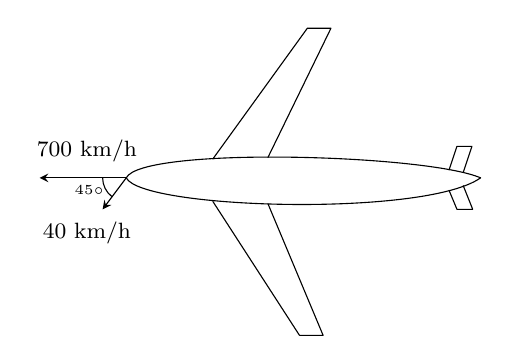
\begin{tikzpicture}[scale=1, font=\footnotesize, line join=round, line cap=round, >=stealth]

			\draw (-4,0.5) .. controls (-3.8,0.9) and (-0.2,0.8) .. (0.5,0.5);

			\draw (-4,0.5) .. controls (-3.8,0.1) and (-0.2,0) .. (0.5,0.5);


			\draw (-2.9,0.74) -- (-1.7,2.4)--(-1.4,2.4)--(-2.2,0.76);

			\draw (-2.9,0.2)--(-1.8,-1.5) --(-1.5,-1.5)-- (-2.2,0.17) ;
			\draw (0.1,0.6)--(0.2,0.9)--(0.39,0.9) --(0.28,0.57);

			\draw (0.1,0.34)--(0.2,0.1)--(0.4,0.1)--(0.28,0.4);
			\draw [->] (-4,0.5)--(-5.1,0.5);


			\node [above] at (-4.5,0.58) {$700$ km/h};
			\draw [->] (-4,0.5)--(-4.3,0.1);

			\node at (-4.5,-0.2) {$40$ km/h};
			\node at (-4.47,0.34) {\tiny $45 \circ$ };
			\draw (-4.3,0.5) arc (180:233:0.3);
	\end{tikzpicture}}
\loigiai{
	\immini{Gọi $v$ là vận tốc máy bay sau khi gặp gió thổi, $\overrightarrow{v}$ là hướng bay của máy bay sau khi gặp gió thổi.\\
	Theo quy tắc hình bình hành ta có $\overrightarrow{v}=\overrightarrow{v}_1+\overrightarrow{v}_2$.\\
	Suy ra
	\allowdisplaybreaks
	\begin{eqnarray*}
		\left|\overrightarrow{v}\right|&=&\left|\overrightarrow{v}_1+\overrightarrow{v}_2\right|=\sqrt{\left(\overrightarrow{v}_1+\overrightarrow{v}_2\right)^2}\\
		&=& \sqrt{\overrightarrow{v}_1^2+\overrightarrow{v}_2^2+2\cdot \overrightarrow{v}_1\cdot \overrightarrow{v}_2\cos\left(\overrightarrow{v}_1,\overrightarrow{v}_2\right)}\\
		&=& \sqrt{700^2+40^2+2\cdot700\cdot40\cdot\cos45^\circ}\\
		&\approx& 728{,}83 ~\text{(km/h).}
	\end{eqnarray*}
	Vậy vận tốc mới của máy bay là $728{,}83$ (km/h).}{{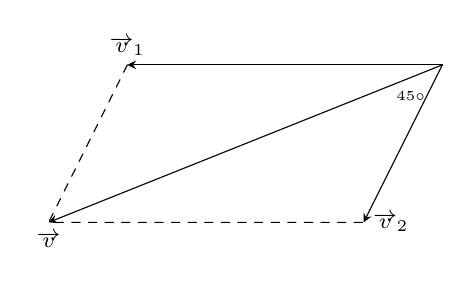
\begin{tikzpicture}[scale=1, font=\footnotesize, line join=round, line cap=round, >=stealth]
			\draw [->] (0,0)--(-4,0)node[above]{$\overrightarrow{v}_1$};
			\draw [->] (0,0)--(-1,-2)node[right]{$\overrightarrow{v}_2$};
			\draw[dashed] (-4,0)--(-5,-2)--(-1,-2);
			\node at (-0.4,-0.4) {\tiny $45 \circ$ };
			\draw [->] (0,0)--(-5,-2)node[below]{$\overrightarrow{v}$};
\end{tikzpicture}}}
}
\end{bt}

\begin{bt}%[Vô Văn Tự]%[0H2K2-2]
	Cho tam giác $ABC$ có $AB=2$, $AC=3$, $\widehat{BAC}=60^\circ$. Gọi $M$ là trung điểm của đoạn thẳng $BC$. Điểm $D$ thỏa mãn $\overrightarrow{AD}=\dfrac{7}{12}\overrightarrow{AC}$.
	\begin{enumerate}
		\item Tính $\overrightarrow{AB}\cdot \overrightarrow{AC}$.
		\item Biểu diễn $\overrightarrow{AM}$, $\overrightarrow{BD}$ theo $\overrightarrow{AB}$, $\overrightarrow{AC}$.
		\item Chứng minh $AM\perp BD$.
	\end{enumerate}
	\loigiai{
	\immini{
		\begin{enumerate}
			\item $\overrightarrow{AB}\cdot \overrightarrow{AC}=\left|\overrightarrow{AB}\right|\cdot\left|\overrightarrow{AC}\right|\cdot\cos\left(\overrightarrow{AB},\overrightarrow{AC}\right)\\= AB\cdot AC\cdot\cos\widehat{BAC}=2\cdot3\cdot\cos60^\circ=3$.
			\item \begin{itemize}
				\item Vì $M$ là trung điểm $BC$ nên \[\overrightarrow{AM}=\dfrac{1}{2}\left(\overrightarrow{AB}+\overrightarrow{AC}\right)=\dfrac{1}{2}\overrightarrow{AB}+\dfrac{1}{2}\overrightarrow{AC}.\]
				\item Ta có $\overrightarrow{BD}=\overrightarrow{AD}-\overrightarrow{AB}$.\\
				Mà $\overrightarrow{AD}=\dfrac{7}{12}\overrightarrow{AC}$, do đó \[\overrightarrow{BD}=\dfrac{7}{12}\overrightarrow{AC}-\overrightarrow{AB}.\]
			\end{itemize}
			\item Ta có
			\allowdisplaybreaks
			\begin{eqnarray*}
				\overrightarrow{AM}\cdot\overrightarrow{BD} &=& \left(\dfrac{1}{2}\overrightarrow{AB}+\dfrac{1}{2}\overrightarrow{AC}\right)\cdot\left(\dfrac{7}{12}\overrightarrow{AC}-\overrightarrow{AB}\right)\\
				&=& \dfrac{7}{24}\overrightarrow{AB}\cdot\overrightarrow{AC}-\dfrac{1}{2}\overrightarrow{AB}^2+\dfrac{7}{24}\overrightarrow{AC}^2-\dfrac{1}{2}\overrightarrow{AC}\cdot \overrightarrow{AB}\\
				&=& -\dfrac{5}{24}\overrightarrow{AB}\cdot\overrightarrow{AC}+\dfrac{7}{24}AB^2-\dfrac{1}{2}AC^2\\
				&=& -\dfrac{5}{24}\cdot 3+\dfrac{7}{24}\cdot 3^2-\dfrac{1}{2}\cdot 2^2=0.
			\end{eqnarray*}
		Suy ra $\overrightarrow{AM}\perp \overrightarrow{BD}$.\\ Vậy $AM\perp BD$.
	\end{enumerate}}{\begin{tikzpicture}[scale=0.8, font=\footnotesize, line join=round, line cap=round, >=stealth]
			\path
			(0,0) coordinate (B)
			(2,4) coordinate (A)
			(6.5,0) coordinate (C)
			($(B)!0.5!(C)$) coordinate (M)
			($(A)!7/12!(C)$) coordinate (D)
			(intersection of A--M and B--D) coordinate (O);
			;
			\draw [->] (A)--(M);
			\draw [->] (A)--(B);
			\draw [->] (A)--(C);
			\draw
			(A)--(B)--(C)--cycle
			(B)--(D)
			;
			\pic[draw,angle radius=6mm]{angle=B--A--C};
			\pic[draw,angle radius=2mm]{right angle = A--O--D};
			\foreach \p/\g in {A/90, B/135, C/-45, M/-90, D/45}
			\draw[fill=black] (\p) circle (1pt) node[shift=(\g:3mm)] {$\p$};
	\end{tikzpicture}}
	}
\end{bt}



